% Created by tikzDevice version 0.12 on 2019-06-11 18:42:54
% !TEX encoding = UTF-8 Unicode
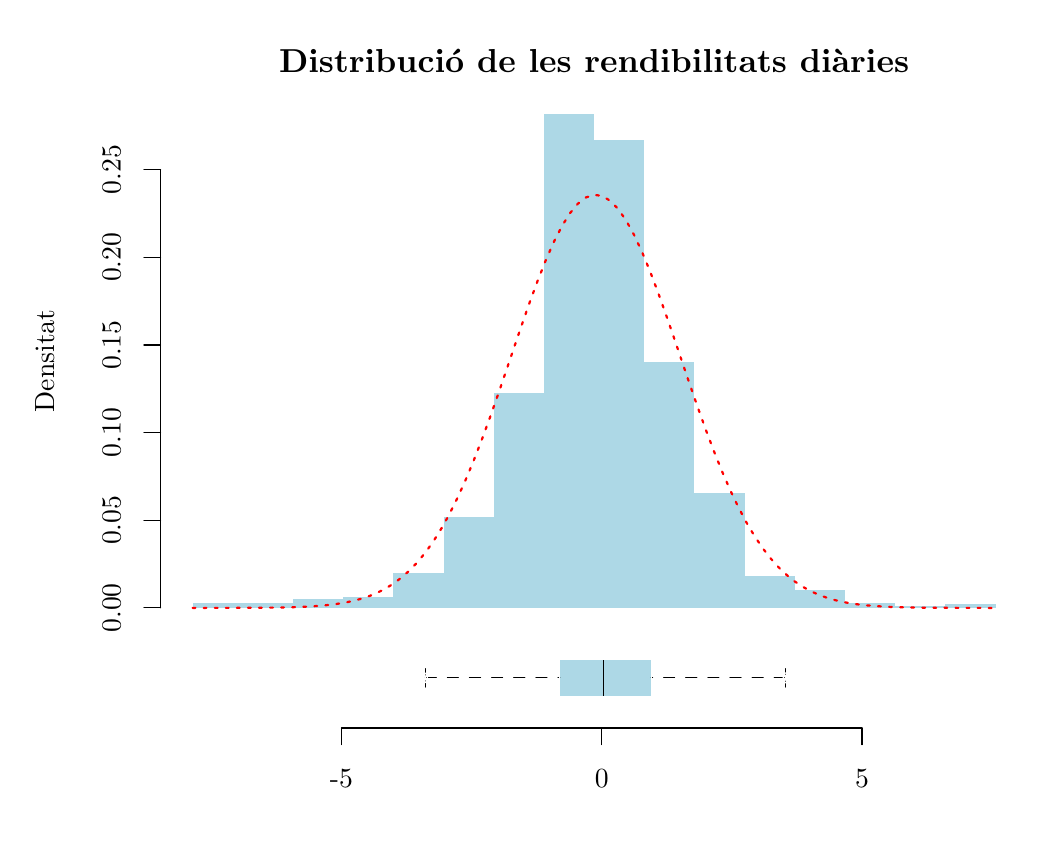
\begin{tikzpicture}[x=1pt,y=1pt]
\definecolor{fillColor}{RGB}{255,255,255}
\path[use as bounding box,fill=fillColor,fill opacity=0.00] (0,0) rectangle (361.35,289.08);
\begin{scope}
\path[clip] ( 48.00, 36.00) rectangle (361.35, 72.27);
\definecolor{fillColor}{RGB}{173,216,230}

\path[fill=fillColor] (192.30, 47.42) --
	(192.30, 60.85) --
	(225.26, 60.85) --
	(225.26, 47.42) --
	cycle;
\definecolor{drawColor}{RGB}{0,0,0}

\path[draw=drawColor,line width= 0.4pt,line join=round] (207.93, 47.42) -- (207.93, 60.85);

\path[draw=drawColor,line width= 0.4pt,dash pattern=on 4pt off 4pt ,line join=round,line cap=round] (143.64, 54.14) -- (192.30, 54.14);

\path[draw=drawColor,line width= 0.4pt,dash pattern=on 4pt off 4pt ,line join=round,line cap=round] (273.78, 54.14) -- (225.26, 54.14);

\path[draw=drawColor,line width= 0.4pt,line join=round,line cap=round] (143.64, 50.78) -- (143.64, 57.49);

\path[draw=drawColor,line width= 0.4pt,line join=round,line cap=round] (273.78, 50.78) -- (273.78, 57.49);
\definecolor{drawColor}{RGB}{255,255,255}

\path[draw=drawColor,line width= 0.4pt,line join=round,line cap=round] (192.30, 47.42) --
	(192.30, 60.85) --
	(225.26, 60.85) --
	(225.26, 47.42) --
	(192.30, 47.42);

\path[draw=drawColor,line width= 0.4pt,line join=round,line cap=round] (105.45, 54.14) circle (  2.25);

\path[draw=drawColor,line width= 0.4pt,line join=round,line cap=round] ( 67.24, 54.14) circle (  2.25);

\path[draw=drawColor,line width= 0.4pt,line join=round,line cap=round] (277.76, 54.14) circle (  2.25);

\path[draw=drawColor,line width= 0.4pt,line join=round,line cap=round] (275.24, 54.14) circle (  2.25);

\path[draw=drawColor,line width= 0.4pt,line join=round,line cap=round] (138.27, 54.14) circle (  2.25);

\path[draw=drawColor,line width= 0.4pt,line join=round,line cap=round] (276.00, 54.14) circle (  2.25);

\path[draw=drawColor,line width= 0.4pt,line join=round,line cap=round] ( 85.71, 54.14) circle (  2.25);

\path[draw=drawColor,line width= 0.4pt,line join=round,line cap=round] (304.50, 54.14) circle (  2.25);

\path[draw=drawColor,line width= 0.4pt,line join=round,line cap=round] (120.46, 54.14) circle (  2.25);

\path[draw=drawColor,line width= 0.4pt,line join=round,line cap=round] (127.44, 54.14) circle (  2.25);

\path[draw=drawColor,line width= 0.4pt,line join=round,line cap=round] (296.66, 54.14) circle (  2.25);

\path[draw=drawColor,line width= 0.4pt,line join=round,line cap=round] (141.54, 54.14) circle (  2.25);

\path[draw=drawColor,line width= 0.4pt,line join=round,line cap=round] (133.52, 54.14) circle (  2.25);

\path[draw=drawColor,line width= 0.4pt,line join=round,line cap=round] (110.29, 54.14) circle (  2.25);

\path[draw=drawColor,line width= 0.4pt,line join=round,line cap=round] (294.39, 54.14) circle (  2.25);

\path[draw=drawColor,line width= 0.4pt,line join=round,line cap=round] (286.35, 54.14) circle (  2.25);

\path[draw=drawColor,line width= 0.4pt,line join=round,line cap=round] (285.74, 54.14) circle (  2.25);

\path[draw=drawColor,line width= 0.4pt,line join=round,line cap=round] (129.37, 54.14) circle (  2.25);

\path[draw=drawColor,line width= 0.4pt,line join=round,line cap=round] (280.86, 54.14) circle (  2.25);

\path[draw=drawColor,line width= 0.4pt,line join=round,line cap=round] (140.10, 54.14) circle (  2.25);

\path[draw=drawColor,line width= 0.4pt,line join=round,line cap=round] ( 78.32, 54.14) circle (  2.25);

\path[draw=drawColor,line width= 0.4pt,line join=round,line cap=round] (302.05, 54.14) circle (  2.25);

\path[draw=drawColor,line width= 0.4pt,line join=round,line cap=round] (289.79, 54.14) circle (  2.25);

\path[draw=drawColor,line width= 0.4pt,line join=round,line cap=round] (346.93, 54.14) circle (  2.25);

\path[draw=drawColor,line width= 0.4pt,line join=round,line cap=round] (125.16, 54.14) circle (  2.25);

\path[draw=drawColor,line width= 0.4pt,line join=round,line cap=round] (349.74, 54.14) circle (  2.25);

\path[draw=drawColor,line width= 0.4pt,line join=round,line cap=round] (314.87, 54.14) circle (  2.25);

\path[draw=drawColor,line width= 0.4pt,line join=round,line cap=round] (298.87, 54.14) circle (  2.25);

\path[draw=drawColor,line width= 0.4pt,line join=round,line cap=round] (129.29, 54.14) circle (  2.25);

\path[draw=drawColor,line width= 0.4pt,line join=round,line cap=round] (102.83, 54.14) circle (  2.25);

\path[draw=drawColor,line width= 0.4pt,line join=round,line cap=round] (128.48, 54.14) circle (  2.25);

\path[draw=drawColor,line width= 0.4pt,line join=round,line cap=round] ( 96.81, 54.14) circle (  2.25);

\path[draw=drawColor,line width= 0.4pt,line join=round,line cap=round] (141.02, 54.14) circle (  2.25);

\path[draw=drawColor,line width= 0.4pt,line join=round,line cap=round] ( 87.03, 54.14) circle (  2.25);

\path[draw=drawColor,line width= 0.4pt,line join=round,line cap=round] (138.12, 54.14) circle (  2.25);

\path[draw=drawColor,line width= 0.4pt,line join=round,line cap=round] (283.11, 54.14) circle (  2.25);

\path[draw=drawColor,line width= 0.4pt,line join=round,line cap=round] (137.35, 54.14) circle (  2.25);

\path[draw=drawColor,line width= 0.4pt,line join=round,line cap=round] (133.79, 54.14) circle (  2.25);

\path[draw=drawColor,line width= 0.4pt,line join=round,line cap=round] (132.24, 54.14) circle (  2.25);

\path[draw=drawColor,line width= 0.4pt,line join=round,line cap=round] ( 59.61, 54.14) circle (  2.25);

\path[draw=drawColor,line width= 0.4pt,line join=round,line cap=round] ( 99.44, 54.14) circle (  2.25);

\path[draw=drawColor,line width= 0.4pt,line join=round,line cap=round] (289.52, 54.14) circle (  2.25);

\path[draw=drawColor,line width= 0.4pt,line join=round,line cap=round] (142.19, 54.14) circle (  2.25);

\path[draw=drawColor,line width= 0.4pt,line join=round,line cap=round] (298.33, 54.14) circle (  2.25);

\path[draw=drawColor,line width= 0.4pt,line join=round,line cap=round] (284.40, 54.14) circle (  2.25);

\path[draw=drawColor,line width= 0.4pt,line join=round,line cap=round] ( 72.36, 54.14) circle (  2.25);

\path[draw=drawColor,line width= 0.4pt,line join=round,line cap=round] (135.46, 54.14) circle (  2.25);

\path[draw=drawColor,line width= 0.4pt,line join=round,line cap=round] (329.01, 54.14) circle (  2.25);
\end{scope}
\begin{scope}
\path[clip] (  0.00,  0.00) rectangle (361.35,289.08);
\definecolor{drawColor}{RGB}{0,0,0}

\path[draw=drawColor,line width= 0.4pt,line join=round,line cap=round] (113.40, 36.00) -- (301.47, 36.00);

\path[draw=drawColor,line width= 0.4pt,line join=round,line cap=round] (113.40, 36.00) -- (113.40, 30.00);

\path[draw=drawColor,line width= 0.4pt,line join=round,line cap=round] (207.44, 36.00) -- (207.44, 30.00);

\path[draw=drawColor,line width= 0.4pt,line join=round,line cap=round] (301.47, 36.00) -- (301.47, 30.00);

\node[text=drawColor,anchor=base,inner sep=0pt, outer sep=0pt, scale=  1.00] at (113.40, 14.40) {-5};

\node[text=drawColor,anchor=base,inner sep=0pt, outer sep=0pt, scale=  1.00] at (207.44, 14.40) {0};

\node[text=drawColor,anchor=base,inner sep=0pt, outer sep=0pt, scale=  1.00] at (301.47, 14.40) {5};
\end{scope}
\begin{scope}
\path[clip] (  0.00, 72.27) rectangle (361.35,289.08);
\definecolor{drawColor}{RGB}{0,0,0}

\node[text=drawColor,anchor=base,inner sep=0pt, outer sep=0pt, scale=  1.20] at (204.67,272.94) {\bfseries Distribució de les rendibilitats diàries};

\node[text=drawColor,rotate= 90.00,anchor=base,inner sep=0pt, outer sep=0pt, scale=  1.00] at (  9.60,168.68) {Densitat};
\end{scope}
\begin{scope}
\path[clip] (  0.00,  0.00) rectangle (361.35,289.08);
\definecolor{drawColor}{RGB}{0,0,0}

\path[draw=drawColor,line width= 0.4pt,line join=round,line cap=round] ( 48.00, 79.41) -- ( 48.00,237.75);

\path[draw=drawColor,line width= 0.4pt,line join=round,line cap=round] ( 48.00, 79.41) -- ( 42.00, 79.41);

\path[draw=drawColor,line width= 0.4pt,line join=round,line cap=round] ( 48.00,111.08) -- ( 42.00,111.08);

\path[draw=drawColor,line width= 0.4pt,line join=round,line cap=round] ( 48.00,142.75) -- ( 42.00,142.75);

\path[draw=drawColor,line width= 0.4pt,line join=round,line cap=round] ( 48.00,174.42) -- ( 42.00,174.42);

\path[draw=drawColor,line width= 0.4pt,line join=round,line cap=round] ( 48.00,206.08) -- ( 42.00,206.08);

\path[draw=drawColor,line width= 0.4pt,line join=round,line cap=round] ( 48.00,237.75) -- ( 42.00,237.75);

\node[text=drawColor,rotate= 90.00,anchor=base,inner sep=0pt, outer sep=0pt, scale=  1.00] at ( 33.60, 79.41) {0.00};

\node[text=drawColor,rotate= 90.00,anchor=base,inner sep=0pt, outer sep=0pt, scale=  1.00] at ( 33.60,111.08) {0.05};

\node[text=drawColor,rotate= 90.00,anchor=base,inner sep=0pt, outer sep=0pt, scale=  1.00] at ( 33.60,142.75) {0.10};

\node[text=drawColor,rotate= 90.00,anchor=base,inner sep=0pt, outer sep=0pt, scale=  1.00] at ( 33.60,174.42) {0.15};

\node[text=drawColor,rotate= 90.00,anchor=base,inner sep=0pt, outer sep=0pt, scale=  1.00] at ( 33.60,206.08) {0.20};

\node[text=drawColor,rotate= 90.00,anchor=base,inner sep=0pt, outer sep=0pt, scale=  1.00] at ( 33.60,237.75) {0.25};
\end{scope}
\begin{scope}
\path[clip] ( 48.00, 72.27) rectangle (361.35,265.08);
\definecolor{fillColor}{RGB}{173,216,230}

\path[fill=fillColor] ( 59.61, 79.41) rectangle ( 77.74, 81.30);

\path[fill=fillColor] ( 77.74, 79.41) rectangle ( 95.87, 81.30);

\path[fill=fillColor] ( 95.87, 79.41) rectangle (114.01, 82.57);

\path[fill=fillColor] (114.01, 79.41) rectangle (132.14, 83.20);

\path[fill=fillColor] (132.14, 79.41) rectangle (150.27, 92.03);

\path[fill=fillColor] (150.27, 79.41) rectangle (168.41,112.21);

\path[fill=fillColor] (168.41, 79.41) rectangle (186.54,157.00);

\path[fill=fillColor] (186.54, 79.41) rectangle (204.67,257.94);

\path[fill=fillColor] (204.67, 79.41) rectangle (222.81,248.48);

\path[fill=fillColor] (222.81, 79.41) rectangle (240.94,168.36);

\path[fill=fillColor] (240.94, 79.41) rectangle (259.08,121.05);

\path[fill=fillColor] (259.08, 79.41) rectangle (277.21, 90.77);

\path[fill=fillColor] (277.21, 79.41) rectangle (295.34, 85.72);

\path[fill=fillColor] (295.34, 79.41) rectangle (313.48, 81.30);

\path[fill=fillColor] (313.48, 79.41) rectangle (331.61, 80.04);

\path[fill=fillColor] (331.61, 79.41) rectangle (349.74, 80.67);
\definecolor{drawColor}{RGB}{255,0,0}

\path[draw=drawColor,line width= 0.8pt,dash pattern=on 1pt off 3pt ,line join=round,line cap=round] ( 59.61, 79.41) --
	( 62.51, 79.41) --
	( 65.41, 79.42) --
	( 68.31, 79.42) --
	( 71.21, 79.42) --
	( 74.11, 79.43) --
	( 77.01, 79.44) --
	( 79.92, 79.45) --
	( 82.82, 79.46) --
	( 85.72, 79.49) --
	( 88.62, 79.52) --
	( 91.52, 79.57) --
	( 94.42, 79.63) --
	( 97.32, 79.72) --
	(100.23, 79.84) --
	(103.13, 80.00) --
	(106.03, 80.21) --
	(108.93, 80.50) --
	(111.83, 80.87) --
	(114.73, 81.34) --
	(117.63, 81.95) --
	(120.53, 82.72) --
	(123.44, 83.69) --
	(126.34, 84.89) --
	(129.24, 86.37) --
	(132.14, 88.16) --
	(135.04, 90.33) --
	(137.94, 92.90) --
	(140.84, 95.93) --
	(143.75, 99.47) --
	(146.65,103.54) --
	(149.55,108.19) --
	(152.45,113.42) --
	(155.35,119.25) --
	(158.25,125.66) --
	(161.15,132.62) --
	(164.06,140.09) --
	(166.96,147.99) --
	(169.86,156.23) --
	(172.76,164.69) --
	(175.66,173.24) --
	(178.56,181.73) --
	(181.46,190.00) --
	(184.37,197.87) --
	(187.27,205.18) --
	(190.17,211.74) --
	(193.07,217.41) --
	(195.97,222.05) --
	(198.87,225.52) --
	(201.77,227.75) --
	(204.67,228.68) --
	(207.58,228.27) --
	(210.48,226.54) --
	(213.38,223.54) --
	(216.28,219.35) --
	(219.18,214.07) --
	(222.08,207.83) --
	(224.98,200.79) --
	(227.89,193.12) --
	(230.79,184.99) --
	(233.69,176.56) --
	(236.59,168.02) --
	(239.49,159.50) --
	(242.39,151.16) --
	(245.29,143.12) --
	(248.20,135.47) --
	(251.10,128.30) --
	(254.00,121.68) --
	(256.90,115.62) --
	(259.80,110.15) --
	(262.70,105.28) --
	(265.60,100.99) --
	(268.51, 97.25) --
	(271.41, 94.02) --
	(274.31, 91.28) --
	(277.21, 88.96) --
	(280.11, 87.03) --
	(283.01, 85.43) --
	(285.91, 84.13) --
	(288.82, 83.07) --
	(291.72, 82.23) --
	(294.62, 81.56) --
	(297.52, 81.04) --
	(300.42, 80.63) --
	(303.32, 80.32) --
	(306.22, 80.08) --
	(309.12, 79.90) --
	(312.03, 79.76) --
	(314.93, 79.66) --
	(317.83, 79.59) --
	(320.73, 79.54) --
	(323.63, 79.50) --
	(326.53, 79.47) --
	(329.43, 79.45) --
	(332.34, 79.44) --
	(335.24, 79.43) --
	(338.14, 79.42) --
	(341.04, 79.42) --
	(343.94, 79.42) --
	(346.84, 79.41) --
	(349.74, 79.41);
\end{scope}
\end{tikzpicture}
